% Diagrams for the "{anvl} to the rescue" slide, one page per diagram:
%   1. compiles: R runs one operation at a time, jit() makes one program;
%   2. differentiates: a loss and its gradient, the slope at a point;
%   3. hardware agnostic: the same R code runs on a CPU or an NVIDIA GPU.
% All three share a 5cm x 3.4cm bounding box, so they line up on the slide.
% Build: pdflatex rescue-figures.tex, then
%        pdf2svg rescue-figures.pdf rescue-<name>.svg <page>
\documentclass[tikz, border=2pt]{standalone}
\usepackage[T1]{fontenc}
\renewcommand{\familydefault}{\sfdefault}
\usetikzlibrary{arrows.meta}
\definecolor{accent}{HTML}{107895}

\tikzset{
  every node/.style={font=\small},
  arr/.style={-{Stealth[length=2mm, width=1.6mm]}, thick, draw=black!60},
  op/.style={draw=black!45, fill=black!5, rounded corners=2pt, thick,
    minimum width=1.25cm, minimum height=0.5cm, font=\ttfamily\small},
  ours/.style={draw=accent, fill=accent!12, rounded corners=3pt, very thick},
  lbl/.style={font=\footnotesize\itshape, text=black!60}
}

\begin{document}

% --- 1. compiles --------------------------------------------------------------
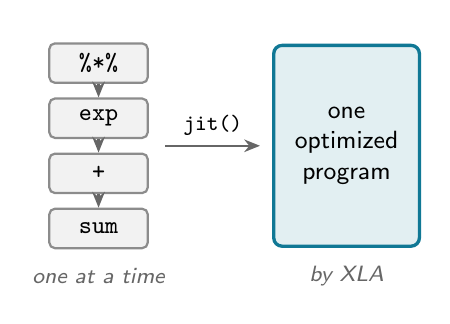
\begin{tikzpicture}
  \path[use as bounding box] (0, 0) rectangle (5, 3.4);
  \node[op] (a) at (0.9, 2.95) {\%*\%};
  \node[op] (b) at (0.9, 2.25) {exp};
  \node[op] (c) at (0.9, 1.55) {+};
  \node[op] (d) at (0.9, 0.85) {sum};
  \draw[arr] (a) -- (b);
  \draw[arr] (b) -- (c);
  \draw[arr] (c) -- (d);
  \node[lbl] at (0.9, 0.25) {one at a time};
  \draw[arr] (1.75, 1.9) -- node[above, font=\ttfamily\footnotesize] {jit()} (2.95, 1.9);
  \node[ours, minimum width=1.85cm, minimum height=2.55cm, align=center]
    at (4.05, 1.9) {one\\optimized\\program};
  \node[lbl] at (4.05, 0.25) {by XLA};
\end{tikzpicture}

% --- 2. differentiates ------------------------------------------------------------
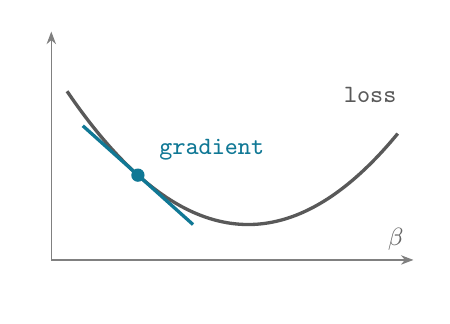
\begin{tikzpicture}
  \path[use as bounding box] (0, 0) rectangle (5, 3.4);
  \draw[-{Stealth[length=1.6mm]}, black!50] (0.3, 0.45) -- (4.9, 0.45) node[above left, text=black!60] {$\beta$};
  \draw[-{Stealth[length=1.6mm]}, black!50] (0.3, 0.45) -- (0.3, 3.35);
  \draw[very thick, black!65, domain=0.5:4.7, smooth, samples=60]
    plot (\x, {0.32 * (\x - 2.8)^2 + 0.9});
  \node[text=black!65, font=\ttfamily\small] at (4.35, 2.55) {loss};
  % The tangent at beta = 1.4: slope 0.64 * (1.4 - 2.8) = -0.896.
  \draw[very thick, accent] (0.7, {1.527 + 0.896 * 0.7}) -- (2.1, {1.527 - 0.896 * 0.7});
  \fill[accent] (1.4, 1.527) circle (2.4pt);
  \node[text=accent, font=\ttfamily\small, anchor=west] at (1.55, 1.85) {gradient};
\end{tikzpicture}

% --- 3. hardware agnostic ---------------------------------------------------------
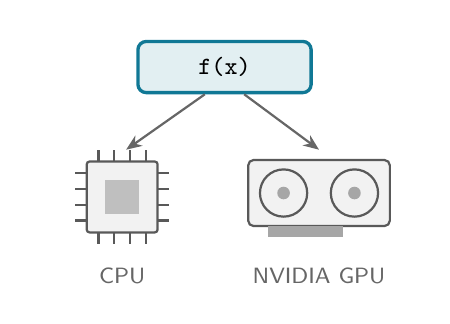
\begin{tikzpicture}
  \path[use as bounding box] (0, 0) rectangle (5, 3.4);
  \node[ours, minimum width=2.2cm, minimum height=0.65cm, font=\ttfamily\small]
    (code) at (2.5, 2.9) {f(x)};
  \draw[arr] (code.south) ++(-0.25, 0) -- (1.25, 1.85);
  \draw[arr] (code.south) ++(0.25, 0) -- (3.7, 1.85);
  % CPU: a chip with pins on all four sides.
  \begin{scope}[shift={(1.2, 1.25)}]
    \draw[thick, black!65, fill=black!5, rounded corners=1pt] (-0.45, -0.45) rectangle (0.45, 0.45);
    \fill[black!25] (-0.22, -0.22) rectangle (0.22, 0.22);
    \foreach \p in {-0.3, -0.1, 0.1, 0.3} {
      \draw[thick, black!65] (\p, 0.45) -- (\p, 0.6);
      \draw[thick, black!65] (\p, -0.45) -- (\p, -0.6);
      \draw[thick, black!65] (0.45, \p) -- (0.6, \p);
      \draw[thick, black!65] (-0.45, \p) -- (-0.6, \p);
    }
  \end{scope}
  \node[lbl, font=\footnotesize] at (1.2, 0.25) {CPU};
  % GPU: a card with two fans and a connector.
  \begin{scope}[shift={(3.7, 1.3)}]
    \draw[thick, black!65, fill=black!5, rounded corners=2pt] (-0.9, -0.42) rectangle (0.9, 0.42);
    \foreach \x in {-0.45, 0.45} {
      \draw[thick, black!65] (\x, 0) circle (0.3);
      \fill[black!35] (\x, 0) circle (0.08);
    }
    \fill[black!35] (-0.65, -0.42) rectangle (0.3, -0.56);
  \end{scope}
  \node[lbl, font=\footnotesize] at (3.7, 0.25) {NVIDIA GPU};
\end{tikzpicture}

\end{document}
